% =============================================================
% Select build mode from:
%     quick - try to compile quickly (no extras, remove front pages)
%     debug - add grid lines/compile times (print variables)
%     proof - local version of "final"
%     final - Final publishable version (calls PurdueThesis - requires LuaLaTeX)
\def\ZZbuildmode{final}
% ==============================================================
% Input arguments required by PurdueThesis
\input{./secs/0-template_options/te00-template-options.tex}
% ==============================================================
% Build the document this will select the document class based on :
%    quick/debug/proof - Local simplified PurdueTheiss.cls file
%                final - Official PurdueThesis.cls file
\RequirePackage{ifthen}
\ifthenelse{\equal{\ZZbuildmode}{final}}
{\documentclass{PurdueThesis}}{\documentclass{PurdueThesisNL}}
% ==============================================================
% Set up the latex document w/ imports, definitions, and
% template customizations
\ConfigureBibliography
\input{./secs/0-template_options/te1-project-settings.tex}
\input{./secs/0-template_options/te2-external-packages.tex}
\input{./secs/0-template_options/te3-custom-commands.tex}
\input{./secs/0-template_options/te4-custom-variables.tex}
\input{./secs/0-template_options/te5-custom-colors.tex}
% \input{./secs/0-template_options/te6-acronyms.tex}

% ==============================================================
\input{./ltx_core/ltx_pkgs.tex}
\input{./ltx_core/new_cmds.tex}
% ==============================================================
\bibliography{./secs/n-back/refs.bib}

\begin{document}
\maketitle

% Only include these sections if this is a proof or final version
\ifthenelse{\boolean{quick}}{}{
    \blankpage
    % Statement of Thesis/Dissertation Approval Page
% This page is REQUIRED.  The page should be numbered "2"
% and should NOT be listed in your TABLE OF CONTENTS.

\begin{statement}
    % Delete or add \entry commands as needed for all committe members.
    \entry{Dr.~Bin Yao, Co-chair}{School of Mechanical Engineering}
    \entry{Dr.~Peter H. Meckl, Co-chair}{School of Mechanical Engineering}
    \entry{Dr.~Richard M. Voyles}{Robotics and Automation Chair, University of Texas at Arlington}
    \entry{Dr.~George T.C. Chiu}{School of Mechanical Engineering}
    % There should be one \approvedby command containing the
    % "FORM 9 THESIS FORM HEAD NAME HERE" (from TEMPL, retrieved on 2020-03-01).
    \approvedby{Dr.~Nicole Key}
\end{statement}

    \blankpage
    % Dedication page is optional.
% A name and often a message in tribute to a person or cause.
% References: WEB9 332.

% \ifthenelse{\boolean{quick-or-debug}}{}
{
\begin{dedication}
To my parents, thank you for always encouraging me to pursue hard things. \\
To my wife, Shruthi, thank you for helping me stay true to my promises.
\end{dedication}
}

    \blankpage
    \begin{acknowledgments}
I would like to acknowledge the support of my co-advisors, Professor Bin Yao and Professor Peter H. Meckl, for their consistent guidance, insights, and feedback throughout my PhD studies. I am deeply thankful to Professor Bin Yao for training me in control theory and for his continual encouragement and advice, which were instrumental in bringing this research together. I am grateful for the opportunity to pursue my PhD under his mentorship. I also wish to thank Professor Peter H. Meckl for his steadfast guidance and inspiration in shaping the SCR-ASC modelling and diagnostic research. His support through Research Assistantships during most of my PhD made this work possible. I appreciate his constructive feedback, which was essential in developing my thesis research.

I would like to thank Professor Richard Voyles for providing hardware and laboratory support, as well as for assisting in defining a practical and meaningful research problem related to the Dexterous Hexrotor, my initial project during the PhD program. I am also grateful to Professor George Chiu for his time, thorough review, and valuable suggestions, which enhanced the quality and clarity of this thesis. I would also like to thank the School of Mechanical Engineering for providing TA support during the initial part of my PhD studies.

I am sincerely grateful to Cummins Inc. for providing the data and sponsorship that enabled the SCR-ASC studies. I especially thank David Schmidt for his detailed discussions regarding system architectures, testing procedures, and truck data, which significantly influenced the modelling and diagnostic work. I also appreciate the support, insights, and collaboration of Adam Kidd, Larry Brunner, Tom Nelson, and Lyle Kocher throughout the project. I would like to acknowledge the foundational contributions of Kaushal Kamal Jain, whose earlier work established important groundwork for this research.

Finally, I want to thank my friends and family, especially my wife Shruthi, for their unwavering encouragement, patience, and understanding. Their constant support has been invaluable, and this accomplishment would not have been possible without them.
\end{acknowledgments}

    \blankpage
    % \input{./secs/0-front/4-preface.tex}
    %
    \setcounter{tocdepth}{2}
    \pdfbookmark{TABLE OF CONTENTS}{Contents}
    \tableofcontents
    \listoftables
    \blankpage
    \listoffigures
    % ===
    % Symbols, Abbreviations, Nomenclature

\begin{symbols}
        $\con{\bullet}$ \ampeq  Concentration of species $\bullet$ (e.g., $[NO_x]$ is concentration of NOx)\\
        $\mol{\bullet}$ \ampeq  Moles of species $\bullet$ (e.g., $\mol{NO_x}$ is moles of NOx)\\
        $\Gamma$ \ampeq  Catalyst adsorption site concentration (moles of adsorption sites per unit surface area of catalyst)\\
        $g_{sat}$ \ampeq switching function used for capturing the catalyst switching between unsaturated and saturated states\\
\end{symbols}

% =============================================================

\begin{abbreviations}
        SCR \ampeq  Selective Catalytic Reduction \\
        ASC \ampeq  Ammonia Slip Catalyst \\
        DOC \ampeq  Diesel Oxidation Catalyst \\
        DPF \ampeq  Diesel Particulate Filter \\
        FTP \ampeq  Federal Test Procedure \\
        RMC \ampeq  Ramped Mode Cycle \\
        EO  \ampeq  Engine Out \\
        IUMPR \ampeq In-use Pefformance Ratio \\
\end{abbreviations}

% =============================================================
% Names of the things I created
\begin{nomenclature}
        $\tau-t_s$ Plot \ampeq  Plot of Residence Time vs Sampling Time\\
        Drive Segment   \ampeq  Segment of the truck data that is contiguous in time with no data breaks longer than a minute.\\
        Saturated Catalyst \ampeq  A catalyst in which all adsorption sites are occupied with ammonia.\\
        Unsaturated Catalyst \ampeq  A catalyst in which some adsorption sites are free (not occupied with ammonia).\\
\end{nomenclature}

}

% Optional: Symbols, Abbreviations, Nomenclature, Glossary

% Always include the abstract
\blankpage
\begin{abstract}%
The existing approach to modelling the reaction flows of diesel engine Selective Catalytic Reduction
after-treatment (SCR-ASC) system uses a sequence of Continuously Stirred Tank Reactors (CSTRs) (n-cell models) to
approximate the PDE's that arise from the plug-flow reactions by discretizing in space. This model introduces a
causality reversal in computation of reaction rates in each cell as they become function of outlet concentrations, i.e,
the concentrations of the products after the reaction. This approximation breaks down when the n-cell model is reduced
down to a single-cell in order to have minimal realization of the dynamics. Thus, the CSTR modelling approach requires
multiple cells to appropriately capture the reaction dynamics, increasing the number of states and parameters that need
estimation. Further, it is observed that the sampling time for the measurement signals is larger than the actual
residence time of the reactants in the chamber. Thus, the measurement signals only capture the averaged effects of the
reactions happening in multiple residence times.

Considering these insights, the present work aims to develop a reduced-order nonlinear discrete model from first
principles that can be parametrized into an identifiable model. Instead of discretizing the plug-flow reaction in space,
we first discretize the system in time considering the interplay between the residence time and sampling time. Then the
reaction process dynamics in the SCR chamber is lumped and reduced to a few significant reactions whose effect on
the time evolution of the measurement signals at the inlet and outlet of the chamber is modelled as a set of difference
equations based on the molar conservation of species. These equations are parametrized as the function of inputs and
states using approximate models for physical properties such as rate constant and density based on the operating
conditions of the system. Finally, an identifiable model for the $NO_x$ process dynamics is developed and validated with
the test-cell data.

Further, the model parameters are shown to be sensitive to the catalyst's aging state. Using the paramter estimates and
their statistics, a hypothesis-testing framework based on the Wald test is developed to detect catalyst aging.
The performance of the proposed aging detector is demonstrated using both test-cell data at different aging
levels and real-world data from four long-haul trucks.
\end{abstract}


% For the official template
\setcounter{tocdepth}{2} % Might need this for the official template?
\ifthen{\equal{\ZZbuildmode}{final}}{\setcounter{tocdepth}{2}}
  % Front matter (title, acknowledgements, abstract, etc)
% ============================================================
\cleardoublepage
\chapter{Introduction}

Diesel engine after-treatment systems reduce the concentrations of harmful gases such as $NO_x$ and $CO$ from exhaust
emissions. The Selective Catalytic Reduction (SCR) system reduces the engine-out $NO_x$ into $N_2$ and $H_2O$, using
ammonia from urea dosing in the presence of a catalyst. This catalytic conversion process is regulated to decrease the
levels of ammonia in the exhaust (ammonia slip), through two methods. The first is feedback control, which adjusts the
urea injection rate based on the exhaust $NO_x$ concentrations. The second method involves an additional catalytic
reaction, the Ammonia Slip Catalysis(ASC), which is designed to oxidize any excess ammonia at the end of the SCR bed.
Figure-\ref{fig:exhaust_scheme} shows a schematic of the SCR-ASC system. It is found that $NO_x$-reduction capacity of
the catalyst reduces with time due to hydro-thermal aging and deposition of contaminants such as excess urea, platinum,
sulfur and phosphorous \cite{matsumoto2016model}. The aging of the catalyst leads to increased emissions of $NO_x$ and
ammonia slip, which can result in non-compliance with environmental regulations. A fault detection system for the aging
of the catalyst would provide better control over the maintenance of the system and improve the overall reduction in
emissions.

\begin{figure}[H]
        \centering
        \includegraphics[width=0.75\textwidth]{./figs/1-intro/SCR-ASC_model.png}
        \caption{Schematic of the SCR-ASC system}
        \label{fig:exhaust_scheme}
\end{figure}

Thus, modern diesel after-treatment systems, particularly those that integrate Selective Catalytic Reduction (SCR) with
Ammonia Slip Catalyst (ASC), necessitate advanced on-board diagnostics (OBD) tools for accurate assessment of catalyst
aging. However, the effectiveness of traditional OBD approaches for this purpose has been impeded by the absence of
model validation with real-world catalyst degradation data, the limitations imposed by existing commercial $NO_x$
sensors' cross-sensitivity to ammonia and the absence of ammonia sensors in commercial vehicles.

Numerous studies have been conducted on modeling the SCR-ASC systems and their control \cite{yuan2015diesel}. A
prevalent modeling approach is to approximate the PDE model for the plug flow reaction into a set of ODEs using sequence
of Continuously Stirred Tank Reactors (CSTRs) approximation (\cite{hsieh2011development} , and \cite{nova2014urea}). The
single CSTR approach was first justified in \cite{devarakonda2008adequacy} and a nonlinear model was developed using
these assumptions, which was then linearized for feedback control design (\cite{devarakonda2009model}). With this model,
observers were designed to estimate the states corresponding to the catalyst's storage (\cite{ma2017observer},
\cite{jain2020term}). A method for detecting the catalyst's aging using an observer for the the change in the maximum
storage capacity of the catalyst, modeled as an exponential function of temperature, was also proposed in
\cite{ma2017observer} and \cite{jiang2019hydrothermal}. Alternatively, an onboad diagnostics (OBD) logic for catalyst
aging based on the tailpipe $NO_x$ and ammonia is proposed in \cite{matsumoto2016model} based on the hypthesis of
reduction in adsorption cites and demonstrated on real world trucks. A common theme in these studies is that the system
identification results in a non-convex, nonlinear parameter estimation problem. Moreover, these studies assume the
availability of all the gaseous states at the tail-pipe for state estimation and to eliminate the effects of
cross-sensitivity of the $NO_x$ sensors, which is not always the case in real-world applications as tailpipe ammonia
measurements are not generally available in commercial vehicles. One other fundamental issue with the CSTR model in the
context of sensor sampling is that the discretization of the continuous model does not account for the resisdance time
of the reactants resulting in high sampling frequency requirements that are not feasible in practice. Additionally, the
discretization requires at least two CSTRs to capture the system dynamics and causality \cite{charla2024reduced},
thereby increasing the model order.

An alternative approach to the problem would be discarding the CSTR assumption and modelling the time evolution of the
sensor signals when a "plug" or "parcel" of the exhaust gases flows through the chamber in discrete time considering the
interplay between sampling and residence time of the reactants.

Such a time evolution introduces constraints on the model due to sampling limitations. To capture the transient
dynamics, the sampling time should be significantly smaller than the "residence time" of the reactants inside the
SCR-ASC chamber. If that is not the case, as is the situation with the present available test and truck data, time
integrated states assuming zero-order holds during the transients need to be introduced into the model and the
input-output model can be derived from the resulting state-space model.

The catalyst saturation that is inherently considered in the CSTR approach needs to be explicitly included as separate
mode of the system. The present work developed such a model under catalyst saturation which becomes one of the modes of
the complete switched nonlinear model. Following the model development we present the parameter estimation algorithm
that estimates the parameters of the saturated catalyst model using the real-world data whose operating mode is unknown
and has additional uncertainties due to $NO_x$ sensor's cross-sensitivity to ammonia.

\begin{figure}[H]
    \centering
    \includegraphics[width = 0.9\textwidth]{./figs/1-intro/ModellingApproach.png}
    \caption{Summary of Modelling Approach}
\end{figure}

Finally, we develope a statistical test for detecting the catalyst aging based on the estimated parameters of the
saturated catalyst model. The performance of the proposed aging detector is demonstrated using both test-cell and
real-world truck data.


\input{secs/1-intro/3-cstr/0-cstr.tex}

\chapter{Data Characteristics}
A critical criterion for assessing the validity of a developed model or diagnostic algorithm is its performance on real-world data, whether sourced from controlled experiments or operational vehicles. For this study, Cummins supplied both test-cell and truck data. Test-cell data were obtained by operating the test cell using established standard drive cycles. Truck data were collected from four long-haul trucks over a one-day period, first with fresh (degreened) catalysts and later after catalyst aging.
%===============================================================================
Test-cell data were collected for both aged and degreened catalysts under three established drive cycles:
\begin{enumerate}
        \item Hot Federal Test Procedure (hFTP)
        \item Cold Federal Test Procedure (cFTP)
        \item Ramped Mode Cycle (RMC)
\end{enumerate}
The main distinction among these three cycles is the operating temperature during the drive cycles (Figure~\ref{fig::test_cell_temp_profiles}). The RMC test operates at higher temperatures than the FTP tests. Although hFTP and cFTP have overlapping temperature ranges, cFTP starts at a much lower temperature. Table~\ref{tab::test_cell_data_vars} summarizes the variables included in the test-cell data.
%==
\begin{figure}[!ht]
        \centering
        \includegraphics[width=0.7\textwidth]{./figs/2-data/test_cell_temp_range.png}
        \caption{Drive Cycle Temperature Profiles of Test Cell Data}
        \label{fig::test_cell_temp_profiles}
\end{figure}
%==
\begin{table}[!ht]
\centering
\caption{Test Cell Data Variables}
\label{tab::test_cell_data_vars}
\begin{tabular}{l l l l}
   \hline \hline
   Data Name &
   Units &
   Variable &
   Description \\ \hline \hline
   %==========================================================================
   LOG\_TM &
   sec &
   $t$ &
   Time
   \\
   %==========================================================================
   EXHAUST\_FLOW &
   kg/min &
   $F$ &
   Exhaust Flow Rate
   \\
   %==========================================================================
   V\_AIM\_TRC\_DPF\_OOUT &
   $\lx{^o}{C}$ &
   $T_{in}$ &
   DPF-out (SCR-in) Gas Temperature
   \\
   % =========================================================================
   V\_AIM\_TRC\_SCR\_OUT &
   $\lx{^o}{C}$ &
   $T_{out}$ &
   SCR/ASC out Gas Temperature
   \\
   % ==========================================================================
   V\_UIM\_FLM\_ESTUREAINJRATE &
   ml/s &
   $u_{inj}$ &
   DEF (Urea Sol.) Dosing Rate
   \\
   % ==========================================================================
   ENG\_CW\_NOX\_FTIR\_COR\_U2 &
   ppm &
   $\con{NO_x}^{out}$ &
   Engine-Out $NO_x$
   \\
   % ==========================================================================
   EXH\_CW\_NOX\_COR\_U1 &
   ppm &
   $\con{NO_x}^{in}$ &
   Tailpipe $NO_x$
   \\
   % ==========================================================================
   EXH\_CW\_AMMONIA\_MEA &
   ppm &
   $\con{NH_3}^{out}$ &
   Tailpipe $NH_3$
   \\
   % ==========================================================================
   EONOX\_COMP\_VALUE &
   ppm &
   $\con{NO_x}^{in}$ &
   Engine-out $NO_x$
   \\
   % ==========================================================================
   V\_SCM\_PPM\_SCR\_OUT\_NOX &
   ppm &
   $\con{NO_x}^{out}_{\chi}$ &
   SCR-out $NO_x$ (cross-sensitive)
   \\
   \hline \hline
\end{tabular}
\end{table}
% =====
A key advantage of test-cell data is the inclusion of FTIR (Fourier Transform Infrared Spectroscopy) sensor measurements, which can estimate both NOx and NH3 gas concentrations. In contrast, the commercial NOx sensor is cross-sensitive to ammonia, whereas FTIR measurements do not exhibit this limitation. The sensor sampling frequency for the test-cell data is 5 Hz (ts = 0.2 s).

%===============================================================================
% =============================================================
\begin{table}[!ht]
\centering
\caption{Truck Data Variables}
\label{tab::truck_data_variables}
\begin{tabular}{l l l l}
\hline \hline
Data Name & Units & Variable & Description \\ \hline \hline
\hline \hline
tod & s & $t$ & Time\\
pSCRBedTemp & $\lx{^o}{C}$ & $T$ & SCR-in Gas Temperature\\
pExhMF & g/s & $F$ & Exhaust Flow Rate\\
pUreaDosing & ml/sec & $u_{inj}$ & DEF (Urea Sol.) Dosing Rate\\
pNOxOutppm & ppm & $\con{NO_x}^{out}_{\chi}$ & Tailpipe $NO_x$ (cross-sensitive)\\
pNOxInppm & ppm & $\con{NO_x}^{in}$ & Engine-Out $NO_x$\\
\hline
\hline
\end{tabular}
\end{table}
% =============================================================

In contrast, the truck data comprise on-board sensor measurements from four long-haul trucks collected during the study
period (Table~\ref{tab::truck_data_mileage}). FTIR sensor measurements for species concentrations and tailpipe ammonia
measurements are not available. The data sampling frequency is 1 Hz. The operating temperatures
(Figure~\ref{fig::truck_data_temp_profiles}) recorded in the truck data range from 200 to 300 $\lx{^o}{C}$, which is similar to
the hFTP drive cycles of the test-cell data. However, the inlet and outlet $NO_x$ concentrations and urea dosing
dynamics more closely resemble those observed in the RMC cycles. The truck data variables are summarized in
Table~\ref{tab::truck_data_variables}.
%===
\begin{figure}[!ht]
    \centering
    \includegraphics[width=0.8\textwidth]{./figs/2-data/truck_temperature_range.png}
    \caption{Temperature Profiles of Truck Data}
    \label{fig::truck_data_temp_profiles}
\end{figure}
%====

The low sampling frequency and absence of ammonia measurements present significant challenges for developing a model of
the reacting flow dynamics and for identifying model parameters. Furthermore, the model's nonlinearity results in the
capture of dynamics at different frequencies due to discrepancies in sampling rates between truck and test-cell data.
This issue can be mitigated by downsampling the test-cell data to 1 Hz, leading to the loss of high-frequency dynamic
information. Conversely, upsampling the truck data is not feasible because the missing high-frequency information cannot
be recovered through interpolation.

\begin{table}[!ht]
        \centering
        \caption{Truck Data Set Years and Mileage Difference}
        \label{tab::truck_data_mileage}
        \begin{tabular}{c c c c}
        \hline \hline
         Truck    & Earlier Data & Latter Data & Mileage \\
         Code     &  Year            & Year    & Difference\\ \hline \hline
        Truck A & $2015$ & $2017$ & $2.8 \times 10^5$\\
        Truck B & $2015$ & $2018$ & $11.9 \times 10^5$\\
        Truck C & $2015$ & $2017$ & $5.9 \times 10^5$\\
        Truck D & $2015$ & $2016$ & $6.6 \times 10^5$ \\
        \hline \hline
        \end{tabular}
\end{table}

% Truck Mapping
% Truck A - AD Transport (adt)
% Truck B - Mesilla Valley (mes)
% Truck C - Werner (wer)
% Truck D - Transwest (trw)
% =====


% ===============================================================================
\section{Residence Time}
A significant challenge posed by low sampling rates is their impact on the residence time of the reacting flow.
Residence time is defined as the total duration a fluid parcel remains within a control volume, such as the SCR-ASC
chamber. For a group of parcels, the frequency distribution of their residence times, known as the residence time
distribution (RTD), characterizes this parameter. In both truck and test-cell datasets, the mode of the residence time
distribution serves as a more appropriate measure of central tendency due to substantial variations in flow rate. The
residence time ($\tau_{mode}$) can be approximated by the formula:
\begin{align}
        \tau_{mode} = \frac{\rho V_{scr}}{F_{mode}}
\end{align}
Where, $\rho$ is the density of the exhaust gas, $V_{scr}$ is the volume of the SCR-ASC chamber, and $F_{mode}$ is the
mode of the mass flow rate of the exhaust gas. We have the dimensions of the SCR-ASC chamber tabulated in
Table~\ref{tab::scr_asc_dimensions} \cite{jain2023model}.
\begin{table}[!ht]
    \centering
    \caption{SCR-ASC Chamber Dimensions}
    \label{tab::scr_asc_dimensions}
    \begin{tabular}{l l}
        \hline \hline
        Parameter & Value \\
        \hline \hline
        Length of SCR & 9.5 in (24.13 cm)\\
        Length of ASC & 2 in (5.08 cm)\\
        Diameter of Chamber & 13 in (33.02 cm)\\
        Volume of SCR-ASC Chamber & 25013.543 $cm^3$\\
        \hline \hline
    \end{tabular}
\end{table}
An additional approximation assumes constant exhaust gas density across the dataset to estimate residence time. The
purpose of this analysis is to demonstrate that the mode residence time is substantially lower than the sampling
interval, despite computational inaccuracies.
\begin{align}
        \rho \approx 1.2 e-3 \, g/cm^3 \quad \text{at} \quad 250 \lx{^o}{C} \\
        \tau^{test}_{mode} = 0.072 \,s \qquad
        \tau^{truck}_{mode} = 0.071 \,s
\end{align}
The similarity in the mode of residence time for both truck and test-cell datasets indicates comparable flow rate
characteristics. The residence time is much shorter than the sensor sampling intervals. Calculations show that the mode
of residence time is approximately $0.07 \, s$, which is less than half the sampling interval for the test-cell data
(0.2 s) and less than one-tenth of the truck data sampling interval ($t_s = 1 \,s$). As a result, measurement signals
for gas concentrations fail to capture reaction transients that occur on time scales shorter than the mean residence
time. This limitation is evident in the $\tau-t_s$ plot (Figure~\ref{fig::tau_ts_res}), where the residence time modes
from the data and the validity regions for the CSTR model do not coincide. Therefore, it is necessary to develop an
"averaged" nonlinear ARMAX model that represents system dynamics at the sampling interval and accounts for the
integrating or memory effects of catalyst storage at the end of each residence time within the sample.
\begin{figure}[!ht]
        \centering
        \includegraphics[width=0.8\textwidth]{./figs/2-data/res_times.png}
        \caption{Residence Times of the Test-cell and Truck Data Sets on the $\tau-t_s$ Plane}
        \label{fig::tau_ts_res}
\end{figure}

%==============================================================================
\section{Data Units}
The available test and truck data used for evaluating the model structure must be converted to common units. The
following table lists the units used for each of the physical properties.
\begin{table}[!ht]
   \centering
   \caption{Measurement Units used in the Model}
   \begin{tabular}{l l}
       \hline \hline
        \itbf{Property} & \itbf{Unit}\\
        \hline \hline
        Concentration   & $ 10^{-3} \, mol/m^{3}$ \\
        Temperature     & $ \times 10 + 200\,^{\circ}\text{C}$ \\
        Flow Rate   & $\times 10 \, g/s$ \\
        Urea Injection  & $\times 10^{-1}\, ml/s$ \\
        Time            & $s$ \\
        \hline \hline
   \end{tabular}
\end{table}

\subsection{Density of the exhaust gas}
The density of the exhaust flow is assumed to be the density of air at that temperature and ambient atmospheric
pressure. Using the ideal gas law:
\begin{align}
    \rho &= \frac{PM}{R T} = \frac{\mu}{T}
\end{align}
\begin{align*}
    \text{where, } &\\
    P &= \text{Pressure of the exhaust gas (ambient pressure)} = 101.325 \: kPa\\
    M &= \text{Molecular weight of the exhaust gas} = 28.9652 \: g/mol\\
    T &= \text{Temperature of the exhaust gas in Kelvin}\\
    R &= \text{Universal gas constant} = 8.314 \: J/(mol.K)
\end{align*}
\itbf{Note}: $P$ and $M$ are replaced with $(P_1 M_1 + P_2 M_2)$ when humidity of the exhaust gas is considered.
\subsubsection{$\%$ Change in density for the temperature range of operation}
We have,
\begin{align*}
    \frac{\delta \rho}{\rho} &= -\frac{\delta T}{T}
\end{align*}
In general the operating temperature is very high ($250 \,^0 C \approx 500 K$), and most of the data lies in $\pm 100 \, ^0 C$ region. Thus, the maximum change in density is less than $10\%$, whose effect on flow rate is far smaller compared to the change in mass flow rate itself. Thus, density can be assumed to be a constant for this process.
\begin{align}
    \rho &= \rho_0
\end{align}
%%==================
\subsubsection{Sensitivity of density to change in $NO_x$ concentrations}
Let, $P_{NO_x}$ be the partial pressure of $NO_x$ and $P_0$ be the total pressure. Assuming the rest of the gas constituents are similar to that of air, we have the density as:
\begin{align*}
    \rho &= \frac{1}{RT} \lr{ P_{NO_x} M_{NO_x} + (P_0 - P_{NO_x}) M_{air}} = \frac{1}{RT} \lr{ P_{NO_x} \lr{M_{NO_x} - M_{air}} + P_0 M_{air}}\\
    \implies \frac{\partial \rho}{\partial P_{NO_x}} &= \frac{1}{RT} \lr{\lr{M_{NO_x} - M_{air}}}\\
    \implies \frac{\delta \rho}{\rho} &= \frac{\lr{\lr{M_{NO_x} - M_{air}} \delta P_{NO_x}}}{\lr{ P_{NO_x} \lr{M_{NO_x} - M_{air}} + P_0 M_{air}}} \qquad \text{at constant temperature}
\end{align*}
Also,
\begin{align*}
    P_{NO_x} &= P_0 \times \frac{n_{NO_x}}{n_{NO_x} + n_{air}} = P_0 \times \frac{\con{NO_x}}{\frac{n_{NO_x} + n_{air}}{V}} = P_0 \times \frac{\con{NO_x}}{N_a (=1)} \qquad \lrb{\because 1 \, mole = n_{tot}/V}
\end{align*}
Thus,
\begin{align*}
    \frac{\delta \rho}{\rho} &= \frac{\lr{\lr{M_{NO_x} - M_{air}} \delta \con{NO_x}}}{\lr{ \con{NO_x}
 \lr{M_{NO_x} - M_{air}} + M_{air}}}
    \qquad \text{at constant temperature}
\end{align*}
We have,
\begin{align*}
    &M_{NO_x} \approx 46 \, g/mol, \qquad M_{air} \approx 29 \, g/mol
\end{align*}
\begin{align*}
    \implies \frac{\delta \rho}{\rho} &= \frac{\lr{ 17 \delta \con{NO_x}}}{17 \con{NO_x} + 29}
    \qquad \text{at constant temperature}
\end{align*}
The above equation demonstrates that the relative change in density due to relative change in $NO_x$ concentration is insignificant, as the molarity of $NO_x$ itself is small.

% ====

\subsection{Parts-per-million to mol/m$^3$}
The commercial and FTIR sensors use ppm (parts per million) in terms of the mole-fraction for concentration
measurements.
%===
\begin{align}
    1 \, ppm^{\lr{mol}} &= \frac{1 \, mol \text{ of gas}}{10^6 \, mol \text{ of air }}
\end{align}
%===
Thus, this measurement when converted into $mol/m^3$, the temperature of the gas will be essential to get the right
value as the volume of 1 mole of air changes with temperature. Assuming ideal gas behavior,
%===
\begin{align}
    V_{air} &= n_{air} T_{air} \times \frac{V_0}{T_0}
    \label{eqn::V_air}
\end{align}
%===
where, $V_0, T_0$ are the volume and temperature of one mole of air under STP conditions. From literature,
$V_0 = 22.4 L = 22.4 \times 10^{-3} m^3$ and $T_0 = 273.15 K$.
%===
\begin{align*}
    T_{air} &= 273.15 + T\\
    n_{air} &= 10^6
\end{align*}
%===
Thus, volume of $10^6$ moles of air at temperature T,
%===
\begin{align}
    V_{air} &= 10^6 \times \frac{273.15 + T}{273.15} \times 22.4 \times 10^{-3} m^3
            = 22.4 \times 10^{3} \times \frac{273.15 + T}{273.15}
    \qquad \lrb{\because \ref{eqn::V_air}}
\end{align}
%===
Thus, we have the conversion between ppm and $mol/m^3$:
%===
\begin{align}
    x \text{ in } mol/m^3 &= \frac{x \text{ in } ppm }{\text{Volume of } 10^6 \text{ moles of air}}
                            = \frac{x \text{ in } ppm}{22.4 \times \lr{\frac{273.15 + T}{273.15}}}
                                \times 10^{-3} \, mol/m^3
\end{align}
%===

% =============================================================================
\section{$NO_x$ Sensor Cross-sensitivity}
Commercial $NO_x$ sensors are cross-sensitive to tailpipe ammonia. The resulting error is modelled as a function of
ammonia concentration and a temperature-dependent cross-sensitivity factor $\chi(T)$. This introduces a non-negative
directional error $\lr{\varepsilon_\chi}$ into the tailpipe $NO_x$ measurement $\con{NO_x}^{out}_{\chi}$
(Figure~\ref{fig::cross_sen_ref1}).
\begin{align}
        \varepsilon_\chi= \chi\lr{T(k)} \times \con{NH_3}^{out}\geq 0
\end{align}
%===
\begin{figure}[!ht]
        \centering
        \includegraphics[width=\figWidth]{./figs/2-data/cross_aged_hftp.png}
        \caption{$NO_x$ sensor cross-sensitivity to tailpipe ammonia}
        \label{fig::cross_sen_ref1}
\end{figure}
The FTIR sensor also has a bias that is directional.

\subsection{$NO_x$ sensor cross-sensitivity Estimation}
The sensor cross-sensitivity $\chi$ can be estimated using the FTIR (Fourier transform infrared) sensor data ($x_1$)
along with the actual sensor measurement data ($y_1$) and the ammonia concentration measurement ($x_2$). We have,
\begin{align*}
    y_1 &= x_1 + \chi x_2
\end{align*}
Note that the FTIR sensor has bias (and drift) that have to be corrected for. Let $x_b$ be the biased sensor data and
$b$ be the bias.
\begin{align*}
    x_b &= x + b(t)
\end{align*}
\subsubsection{Bias correction}
The value of $b$ is assumed to linearly change with time: this assumption captures the linear drift in the sensor as
well.
\begin{align*}
    b(t) &= b_1 t + b_0
\end{align*}
$b_1$ and $b_0$ are estimated using the bias at the starting segment and the tail end of the data can fit the change
linearly with time.
\begin{figure}[!ht]
    \begin{minipage}{0.49\textwidth}
        \begin{figure}[H]
            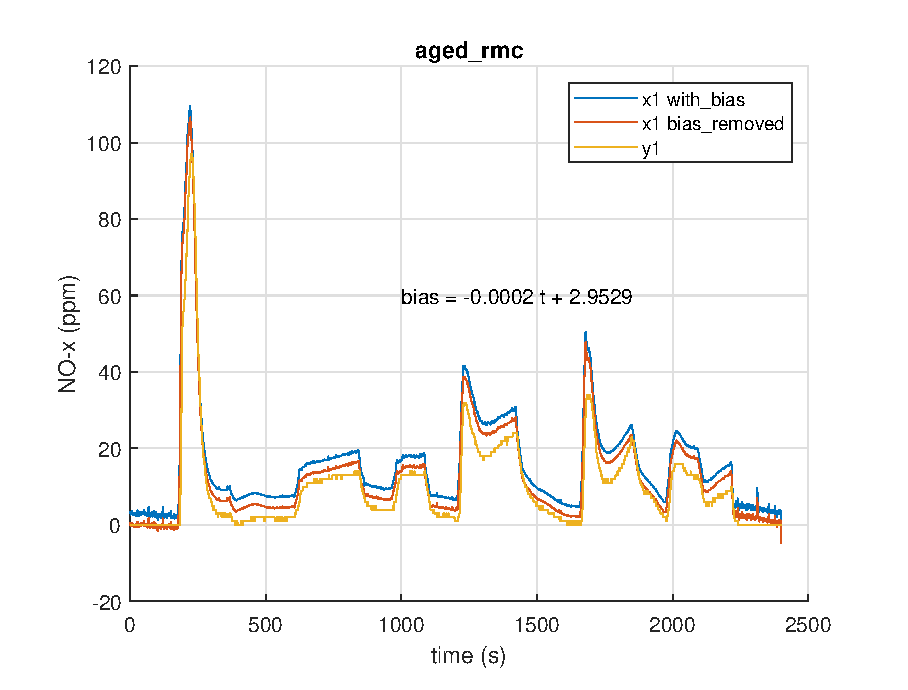
\includegraphics[width=\textwidth]{./figs/2-data/chi_est/aged_rmc_NOx_bias.eps}
        \end{figure}
    \end{minipage}
    \begin{minipage}{0.49\textwidth}
        \begin{figure}[H]
            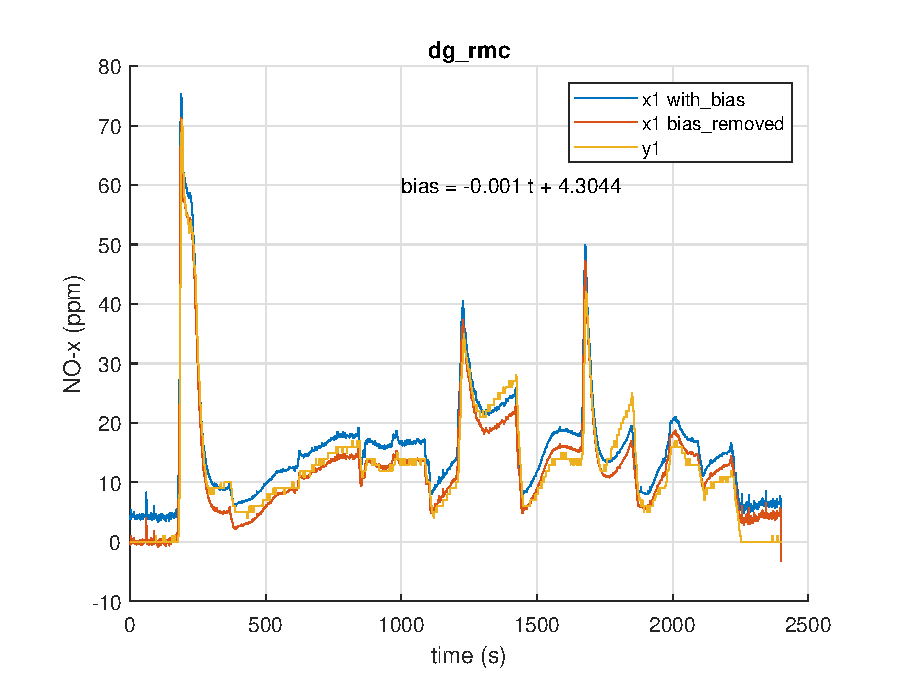
\includegraphics[width=\textwidth]{./figs/2-data/chi_est/dg_rmc_NOx_bias.eps}
        \end{figure}
    \end{minipage}
        \caption{Sensor bias correction for RMC cycles}
        \label{fig::bias_corr}
\end{figure}
The results depicted in Figure~\ref{fig::bias_corr} indicate that the coefficient of \( t \), \( b_1 \) (drift), is
considerably smaller in comparison to the bias \( b_0 \), suggesting it can be disregarded.

\subsubsection{Effect of $NH_3$ sensor bias and minimum threshold for cross-sensitivity}
The ammonia sensor used for ammonia measurement also has bias and there is a threshold on ammonia for which the $NO_x$
sensor becomes cross-sensitive to ammonia. Thus the expression for cross-sensitivity becomes:
\begin{align*}
    y_1 &= \lr{x_1 - b_0} + \chi (x_2 - b_{th})\\
\end{align*}

\subsubsection{Least-squares estimation assuming temperature independence}
The temperature changes in the RMC cycle do not affect the cross-sensitivity factor significantly. Thus, it can be treated as
a constant with respect to temperature fluctuations in that range. We have,
\begin{align*}
    \underbrace{y_1 - x_1}_{\pmb y} &= \underbrace{\bm{x_2 & -1}}_{\pmb \phi^T} \underbrace{\bm{ \chi \\ \underbrace{\chi b_{th} + b_0}_{=b}}}_{ \pmb \theta}\\
\end{align*}
Using the above model, the least-squares estimation of $\chi$ and $b$ is performed for RMC cycles. The results are shown
in Figure~\ref{fig::chi_est} and the error in estimation is shown in Figure~\ref{fig::chi_error}.
\begin{figure}[!ht]
    \begin{minipage}{0.49\textwidth}
        \begin{figure}[H]
            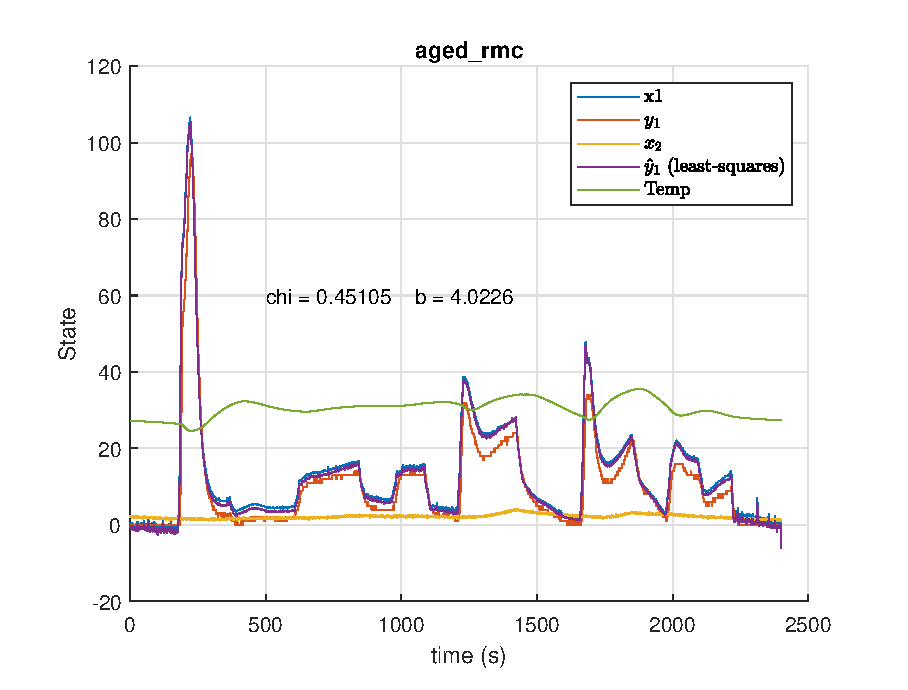
\includegraphics[width=\textwidth]{./figs/2-data/chi_est/aged_rmc_chi.eps}
        \end{figure}
    \end{minipage}
    \begin{minipage}{0.49\textwidth}
        \begin{figure}[H]
            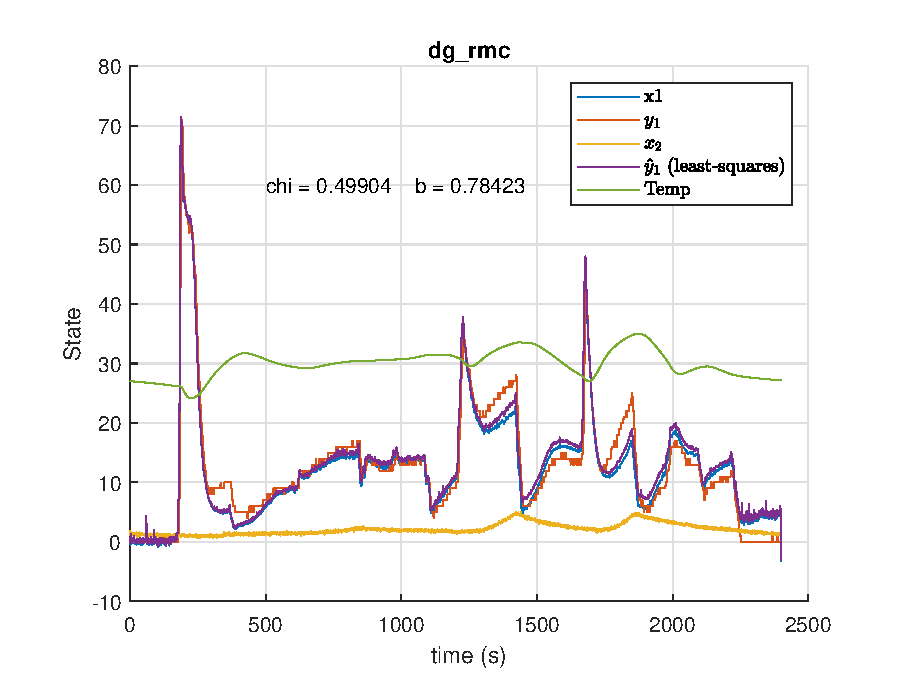
\includegraphics[width=\textwidth]{./figs/2-data/chi_est/dg_rmc_chi.eps}
        \end{figure}
    \end{minipage}
        \caption{$\chi$ estimation for RMC cycles}
        \label{fig::chi_est}
\end{figure}
\begin{figure}[!ht]
    \centering
    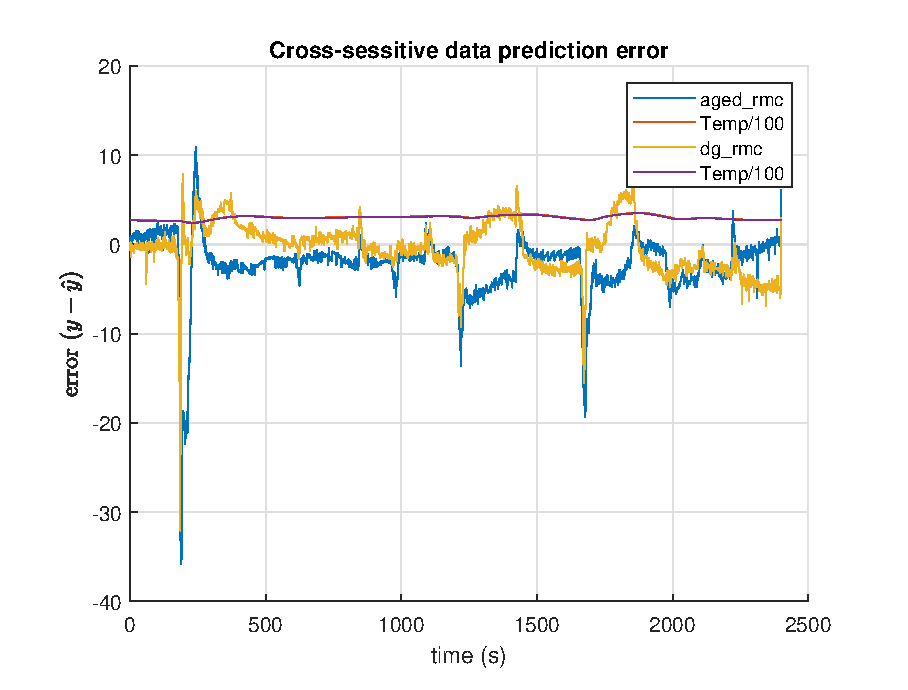
\includegraphics[width = 0.5 \textwidth]{./figs/2-data/chi_est/chi_error.eps}
    \caption{Error in $\chi$ estimation}
    \label{fig::chi_error}
\end{figure}
The error can be reduced by introducing the effects of temperature into $\chi$.

\subsubsection{Least-squares estimation with $\chi$ as a temperature function}
For simplicity, $\chi$ is assumed to be a linear function of temperature.
\begin{align*}
    \chi(T) &= a T - b_T
\end{align*}
Assuming the sensor-bias is not time-varying ($\because$ $b_1$ is small). The sensor bias, cross-sensitivity threshold
and temperature dependence can be combined into:
\begin{align*}
    y_1 &=  \lr{x_1 - b_0} + \lr{aT - b_{T}} \lr{x_2 - b_{th}}\\
    \lr{y_1 - x_1} &= a T x_2 - a b_{th} T - b_{T} x_2 + (b_T b_{th} - b_0)\\
    \underbrace{y_1 - x_1}_{\pmb y} &= \underbrace{\bm{T x_2 & -T & -x_2 & 1}}_{\pmb \phi^T} \underbrace{\bm{a \\ a b_{th} \\ b_T \\ b_T b_{th} - b_0}}_{\pmb \theta}\\
\end{align*}
The least-squares estimation of the parameters is performed using the above model and the results are shown in Figure~\ref{fig::chi_est_T} and the error in estimation is shown in Figure~\ref{fig::chi_error_comp}.
\begin{figure}[!ht]
    \begin{minipage}{0.49\textwidth}
        \begin{figure}[H]
            \includegraphics[width=\textwidth]{./figs/2-data/chi_est/aged_rmc_chiT.eps}
        \end{figure}
    \end{minipage}
    \begin{minipage}{0.49\textwidth}
        \begin{figure}[H]
            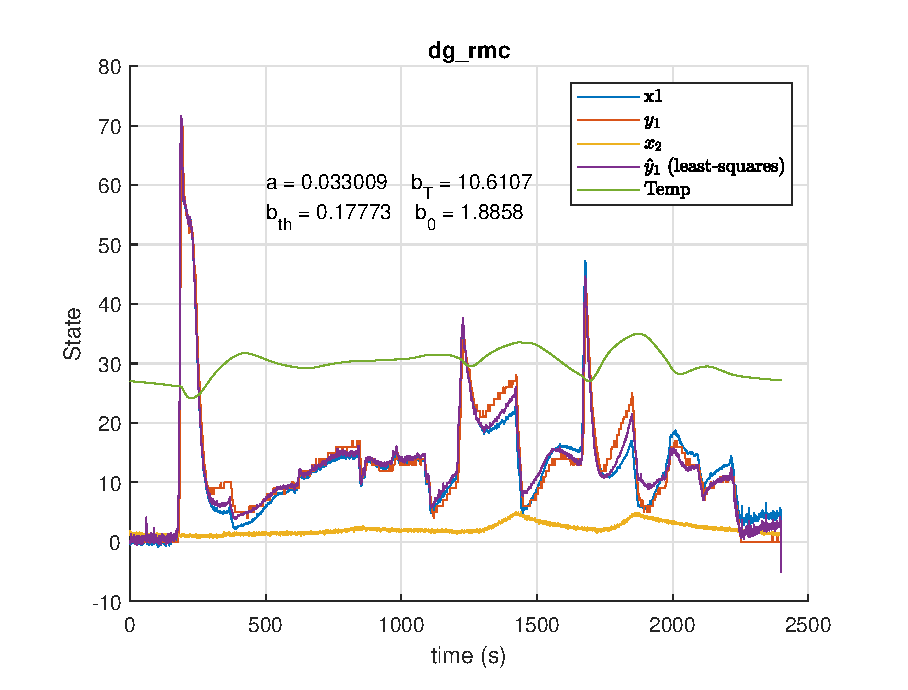
\includegraphics[width=\textwidth]{./figs/2-data/chi_est/dg_rmc_chiT.eps}
        \end{figure}
    \end{minipage}
        \caption{$\chi$ estimation for RMC cycles}
        \label{fig::chi_est_T}
\end{figure}
\begin{figure}[!ht]
    \begin{minipage}{0.49\textwidth}
        \begin{figure}[H]
            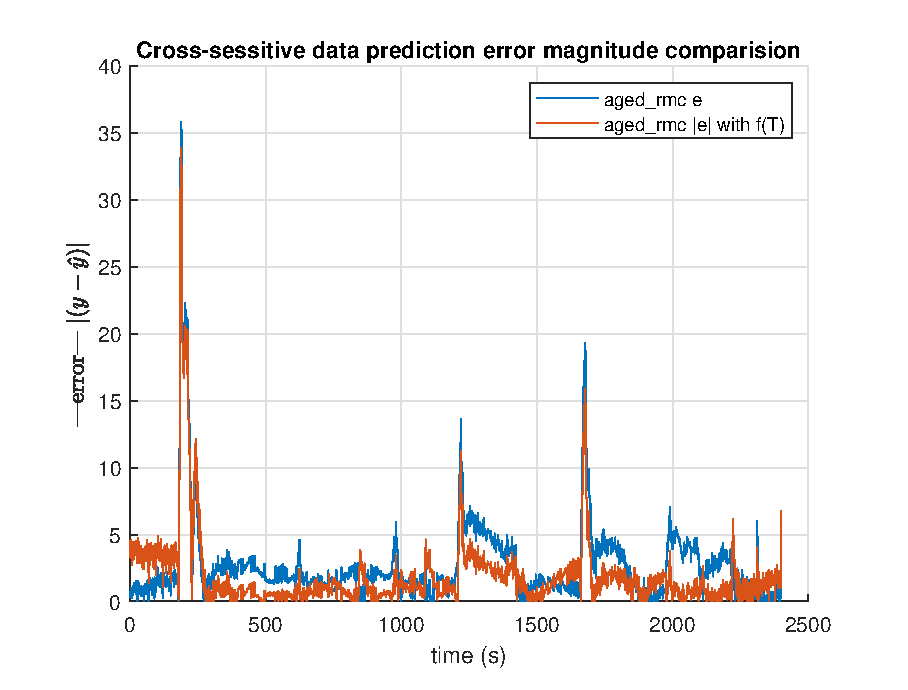
\includegraphics[width=\textwidth]{./figs/2-data/chi_est/aged_error_comp.eps}
        \end{figure}
    \end{minipage}
    \begin{minipage}{0.49\textwidth}
        \begin{figure}[H]
            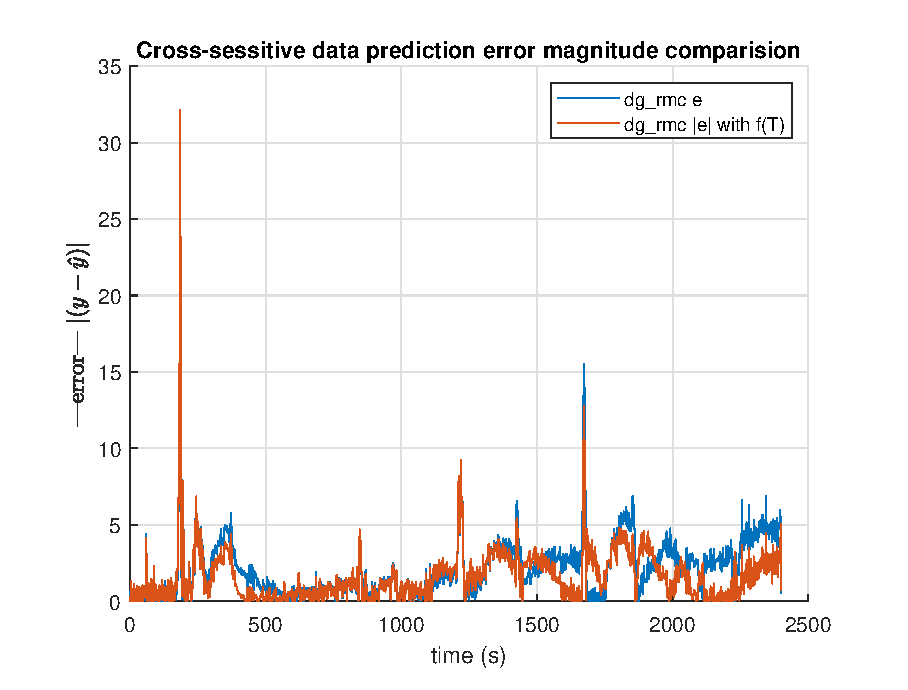
\includegraphics[width=\textwidth]{./figs/2-data/chi_est/dg_error_comp.eps}
        \end{figure}
    \end{minipage}
        \caption{Effect of temperature on prediction errors for $\chi$ estimation in RMC cycles}
        \label{fig::chi_error_comp}
\end{figure}
Introducing temperature clearly decreases the prediction error (Figure~\ref{fig::chi_error_comp}) in the model. However,
the reduction in error, while noticeable, is not significant when compared to the temperature-independent model
(Figure~\ref{fig::chi_error}), whose error remains within acceptable limits. Moreover, tailpipe ammonia measurements are
required for estimation of the cross-sensitivity error. Hence, for the current work, the cross-sensitivity effect is
treated as an unknown bounded disturbance.

% =============================================================================





\section{Data Preprocessing in Test-Cell and Truck Data}



\section{Test-Cell Data Preprocessing}
% \subsection{Test Data Signal Ranges}
The ranges of the measurement signals are tabulated bellow:
\begin{table}[H]
\centering
\begin{tabular}{c c c c c}
\hline \hline
Variable & Units & & & \\
\hline \hline
Degreend Data & & Cold FTP & Hot FTP & RMC\\ \hline
$T$   & $+200 \, ^0C$ & [60.96, -174.0] & [67.38, -64.7] & [148.76, 43.76]
\\
$F$   & $g/s$ & [439.04, 0.0]& [431.14, 0.0]& [403.84, 32.65]
\\
$x_1$ & $mol/m^3$ & [17.24, -2.97] &  [3.55, -0.57]& [2.23, 0.14]
\\
$x_2$ & $mol/m^3$ & [0.06, 0.0] & [0.17, -0.01] & [0.27, 0.06]
\\
$u_1$ & $mol/m^3$ & [20.16, 0.0] & [16.46, 0.0] & [24.26, 0.0]
\\
$u_2$ & $mol/m^3$ & [1.4, 0.0] & [1.0, 0.0] & [0.71, 0.01]
\\
$y_1$ & $mol/m^3$ & [0.07, 0.0]& [0.82, 0.0]& [2.11, 0.0]
\\
\hline
Aged Data & &Cold FTP & Hot FTP & RMC\\ \hline
$T$   & $+200 \, ^0C$ & [67.03, -172.85]& [72.5, -56.35]& [154.38, 48.18]
\\
$F$   & $g/s$ & [416.85, 0.0]& [418.24, 0.0]& [409.59, 32.63]
\\
$x_1$ & $mol/m^3$ & [25.03, 0.01] & [4.9, -0.42] & [3.24, 0.08]
\\
$x_2$ & $mol/m^3$ & [0.04, 0.0] & [0.6, -0.02] & [0.23, 0.08]
\\
$u_1$ & $mol/m^3$ &  [18.58, 0.0]& [16.26, 0.0] & [22.89, 0.0]
\\
$u_2$ & $mol/m^3$ & [1.31, 0.0] & [1.0, 0.0] & [0.67, 0.01]
\\
$y_1$ & $mol/m^3$ & [0.09, 0.0]& [1.06, 0.0]& [2.86, 0.0]
\\
\hline \hline
\end{tabular}
\caption{Test cell data ranges}
\end{table}


%==============================================================================

% \subsection{Signal Processing Steps}
The signal processing steps for getting the viable data used for model validation are summarized bellow.
\begin{figure}[H]
        \centering
        \includegraphics[width = 0.9\textwidth]{./figs/2-data/DataProcessingPipeline.png}
        \caption{Summary of Signal Processing Steps for Test Cell Data}
\end{figure}


% ==============================================================================

\section{Truck Data Preprocessing}
% \subsection{Truck Data Signal Ranges}
The ranges of the measurement signals are tabulated below:
\begin{table}[H]
\centering
\begin{tabular}{c c c c c c}
\hline \hline
Variable & Units & & & & \\
\hline \hline
Degreened Data & & adt\_15 & mes\_15 & wer\_15 & trw\_15 \\ \hline
$T$   & $+200 \, ^0C$ & [135.71, -79.68]& [116.91, -93.05]& [98.7, -142.85]& [125.21, -169.55]
\\
$F$   & $g/s$ & [425.94, 15.82]& [529.08, 0.0]& [386.51, 0.0]& [559.86, 0.0]
\\
$u_1$ & $mol/m^3$ & [27.34, 0.0]& [103.47, -6.87]& [49.99, 0.0]& [100.22, -6.73]
\\
$u_2$ & $mol/m^3$ & [0.89, 0.0]& [1.5, 0.0]& [1.07, 0.0]& [2.18, 0.0]
\\
$y_1$ & $mol/m^3$ & [24.66, 0.0] & [20.86, 0.0] & [22.51, 0.0]& [30.73, 0.0]
\\
\hline
Aged Data & & adt\_17 & mes\_18 & wer\_20 & trw\_16 \\ \hline
$T$   & $+200 \, ^0C$ & [111.04, -150.35]& [173.4, -86.67]& [353.84, -127.68]& [152.48, -155.45]
\\
$F$   & $g/s$ & [440.63, 0.0]& [391.06, 0.0]& [425.77, 0.0]& [569.7, 0.0]
\\
$u_1$ & $mol/m^3$ & [41.76, 0.0]& [36.89, 0.0]& [35.16, 0.0]& [68.93, 0.0]
\\
$u_2$ & $mol/m^3$ & [1.88, 0.0]& [1.07, 0.0]& [1.28, 0.0]& [1.66, 0.0]
\\
$y_1$ & $mol/m^3$ & [9.14, 0.0]& [19.6, 0.0]& [49.99, 0.0]& [38.39, 0.0]
\\
\hline \hline
\end{tabular}
\caption{Truck data ranges}
\end{table}


% =============================================================================

% \subsection{Signal Processing Steps}
The road data was collected from trucks operating in the United States  for two days separated by a few years
(Table~\ref{tab::truck_data_summary}) during which the catalyst has aged based on the existing performance measures. The
data contains measurements of $NO_x$ sensors before and after the catalyst, as well as other required variables
including flow rate, temperature and urea injection rate. The data preporcessing includes,
\begin{enumerate}
        \item removing the rows with missing values,
        \item removing the rows whose operating temperature range is beyond range of $200-300 \,^0C$,
        \item interpolating the missing data if the data breaks are smaller than a minute, and finally,
        \item smooting the data using non-causal chebyshev filter.
\end{enumerate}
The preprocessed data is than partitioned into drive segments with no breaks which correspond to a continuous driving
period from engine start to engine stop.
%===

\chapter{SCR-ASC Reacting Flow Dynamics: Governing Equations}

\chapter{$NO_x$ Reduction Dynamics: Discrete Nonlinear Model}

The discrete nonlinear recursive model that is linear in parameters can be derived from the molar conservation equations
directly using control volume (Figure~\ref{fig::ctrl_vol}). The model derivation involves three main steps:
\begin{figure}[!ht]
        \centering
        \includegraphics[width = 0.5\textwidth]{./figs/4-NOx_mdl/plug_flow_discrete.png}
        \caption{SCR-ASC system abstraction}
        \label{fig::ctrl_vol}
\end{figure}
\begin{enumerate}
        \item We have the molar-conservation equations across the control volume within one residence time.
                \begin{multline}
                        \underbrace{\mol{NO_x}^{out} }_{ \con{NO_x}^{out} \tau F_{vol} } (t + (i+1) \tau) =
                                \underbrace{\mol{NO_x}^{in} }_{ \con{NO_x}^{in} \tau F_{vol} } (t + i \tau)
                                + V_{scr} \int_0^{\tau}
                                                \underbrace{\frac{d}{dt} \con{NO_x}^{scr}}_
                                                        {k_{s2v} k_{scr} \con{NO_x}^{in} \con{NH_3}^{ads}}
                                           dt
                        \label{eqn::nox_bal}
                \end{multline}
                \begin{multline}
                       \mol{NH_3}^{ads} (t + (i+1) \tau) =
                                \underbrace{\mol{NH_3}^{ads} }_{A_{scr} \con{NH_3}^{ads}} (t + i \tau)
                                + A_{scr} \int_0^{\tau}
                                               \frac{d}{dt} \con{NH_3}^{ads}
                                               % \underbrace{}_{
                                               %         - \con{NH_3}^{ads}
                                               %                \lrf{
                                               %                k_{ads} \con{NH_3}^{in}
                                               %                + k_{scr} \con{NO_x}^{in}
                                               %                + k_{od}}
                                               %         + \Gamma k_{ads} \con{NH_3}^{in}
                                               %                }
                                                dt
                        \label{eqn::ads_bal}
                \end{multline}
        \item By summing the equations from (\ref{eqn::nox_bal}) for  $i = 0$ to $n-1$, where $n$ is the total number of residence times within one sampling period $(= t_s/\tau)$, we get the relation between the total number of moles of $NO_x$ that entered, reduced and left the SCR-ASC chamber. Finally, writing the equation in terms of the inlet and outlet concentrations we get the equation relating inlet and outlet concentrations at the end of sampling period as:
                \begin{multline}
                        \underbrace{\con{NO_x}^{out}}_{x_1}(t + t_s) =
                                \underbrace{\con{NO_x}^{in}}_{u_1}(t) - \tau(t) k_{s2v} k_{scr}(t) \con{NO_x}^{in}(t) \underbrace{\lrf{\frac{1}{n} \sum_{i = 0}^{n-1} \con{NH_3}^{ads}(t + i \tau)}}_{\sigma}
                        \label{eqn::nox_avg}
                \end{multline}

        \item The dynamics of $\sigma$, the average surface concentration of adsorbed ammonia on the catalyst in the
                given sampling period, can be obtained by summing the equations from (\ref{eqn::ads_bal}) for $i = 0$ to
                $n-1$ which is the sampling period. This results in a telescopic cancellation of the terms resulting in
                an equation relating the moles in the current sample to the moles in the next sample
                (section~\ref{sec::sigma_deriv}). As the ammonia desorption and ammonia oxidation have the same effect
                ($\sigma$ reduction) on the surface concentration of ammonia the rate constants can
                be lumped by addition, i.e., $k_{od} = k_{oxi} + k_{des}$. We have,
                \begin{multline}
                        \sigma(t + t_s) = \sigma(t) - \sigma(t) t_s \lrf{k_{ads}(t) \con{NH_3}^{in}(t)
                                                                                + k_{scr}(t) \con{NO_x}^{in}(t)
                                                                                + k_{od}(t)}
                                                \\
                                                + \Gamma t_s k_{ads}(t) \con{NH_3}^{in}(t)
                        \label{eqn::ads_avg}
                \end{multline}
        \item Finally, using (\ref{eqn::nox_avg}), $\sigma(t+t_s)$ and $\sigma(t)$ can be eliminated from
                (\ref{eqn::ads_avg}) to get a dynamic model for the $NO_x$-reduction process that explicitly depends
                on the measured inputs and states alone.
                \begin{align}
                        \text{Let }\quad \eta(k) = u_1(k-1) - x_1(k)
                \end{align}
\begin{align}
        \eta(k+1) =& \eta(k) \lrb{\frac{\tau(k)}{\tau(k-1)}}
                                \lrb{\frac{u_1(k)}{u_1(k-1)}}
                                \lrb{\frac{k_{scr}(k)}{k_{scr}(k-1)}} \notag \\
                &-\eta(k) \lrb{\frac{\tau(k)}{\tau(k-1)}}
                                \lrb{\frac{u_1(k)}{u_1(k-1)}}
                                \lrb{\frac{k_{scr}(k)}{k_{scr}(k-1)}}
                t_s k_{ads}(k-1) \con{NH_3}^{in}(k-1)
                \notag \\
                &-\eta(k) \lrb{\frac{\tau(k)}{\tau(k-1)}}
                                \lrb{\frac{u_1(k)}{u_1(k-1)}}
                                \lrb{\frac{k_{scr}(k)}{k_{scr}(k-1)}}
                t_s k_{scr}(k-1) u_1(k-1)
                \notag \\
                &-\eta(k) \lrb{\frac{\tau(k)}{\tau(k-1)}}
                                \lrb{\frac{u_1(k)}{u_1(k-1)}}
                                \lrb{\frac{k_{scr}(k)}{k_{scr}(k-1)}}
                t_s k_{od}(k-1)
                \notag \\
                &+ t_s k_{s2v} \times \lrf{\Gamma(k-1) \tau(k) u_1(k) \con{NH_3}^{in}(k-1)} \times \lr{k_{scr}(k) k_{ads}(k-1)}
                \label{eqn::disc_NOx}
\end{align}

\end{enumerate}

The above equation (\ref{eqn::disc_NOx}) is parametrized using the models for the physical properties and
urea-dosing and used for parameter estimation and validation.

Steps 1, 2 and 3 are discussed in detail in the previous sections. The step-4 derivation is presented below followed by the parametrization.


\section{Modelling using average concentration change of $NO_x$ due to reduction in a sample}
Let, \textbf{$\eta$ denote the change in concentration from inlet to outlet $NO_x$ in one sample}. This is the change in concentration in the exhaust due to the $NO_x$ reduction.
%
\begin{align}
        \eta(k) &= \con{NO_x}^{in}(k-1) - \con{NO_x}^{out}(k) = u_1(k-1) - x_1(k)
\end{align}
%
Thus, rewriting the $NO_x$ process dynamics (\ref{eqn::nox_avg}) in terms of $\eta$, we have,
\begin{align}
        \eta(k+1) &= \tau(k) k_{s2v} k_{scr}(k) u_1(k) \sigma(k)\\
        %===
        \implies \sigma(k) &= \frac{\eta(k+1)}{\tau(k) k_{s2v} k_{scr}(k) u_1(k)}
        \label{eqn::sigma_elim}
\end{align}
%
The above equation (\ref{eqn::sigma_elim}) can be used to eliminate the unknown quantity $(\sigma)$ from equation (\ref{eqn::ads_avg}). We have,
\begin{multline}
        \sigma(k+1) = \sigma(k) - \sigma(k) t_s k_{ads}(k) \con{NH_3}^{in}(t)
                        - \sigma(k) t_s k_{scr}(k) u_1(k)
                        - \sigma(k) t_s k_{od}(k)
                        \\ + \Gamma(k) t_s k_{ads}(k) \con{NH_3}^{in}(k)
\end{multline}
writing the above equation for $\sigma(k)$:
\begin{multline*}
         \sigma(k) = \sigma(k-1)\lrf{1 -  t_s k_{ads}(k-1) \con{NH_3}^{in}(t-1)
                        -  t_s k_{scr}(k-1) u_1(k-1)
                        -  t_s k_{od}(k-1)}
                        \\ + \Gamma(k-1) t_s k_{ads}(k-1) \con{NH_3}^{in}(k-1)
\end{multline*}
Let,
\begin{align}
        \gamma_{proc}(k-1) &= \lrf{1 -  t_s k_{ads}(k-1) \con{NH_3}^{in}(t-1)
                        -  t_s k_{scr}(k-1) u_1(k-1)
                        -  t_s k_{od}(k-1)}
        \label{eqn::gamma_proc}
        \\
        \implies \sigma(k) &= \sigma(k-1) \gamma_{proc}(k-1) + \Gamma(k-1) t_s k_{ads}(k-1) \con{NH_3}^{in}(k-1)
        \label{eqn::sig_gamma_proc}
\end{align}
Eliminating $\sigma(k)$ and $\sigma(k-1)$ from the above equation (\ref{eqn::sig_gamma_proc}) using equation (\ref{eqn::sigma_elim}):
\begin{multline*}
        \frac{\eta(k+1)}{\tau(k) k_{s2v} k_{scr}(k) u_1(k)}
        = \frac{\eta(k)}{\tau(k-1) k_{s2v} k_{scr}(k-1) u_1(k-1)} \times \gamma_{proc}(k-1)\\
                        \\ + \Gamma(k-1) t_s k_{ads}(k-1) \con{NH_3}^{in}(k-1)
\end{multline*}
Thus, we have the recursive equation for change in concentration due to reduction:
\begin{multline}
        \eta(k+1) = \eta(k) \times \lr{\frac{\tau(k)}{\tau(k-1)}}
                                \times \lr{\frac{u_1(k)}{u_1(k-1)}}
                                \times \lr{\frac{k_{scr}(k)}{k_{scr}(k-1)}}
                                \times \gamma_{proc}(k-1)
                                \\
                        + t_s k_{s2v} \times \lrf{\con{NH_3}^{in} \Gamma(k-1) \tau(k) u_1(k)} \times \lr{k_{scr}(k) k_{ads}(k-1)}
\end{multline}
Explicitly writing the individual terms:
\begin{align*}
        \eta(k+1) =& \eta(k) \lrb{\frac{\tau(k)}{\tau(k-1)}}
                                \lrb{\frac{u_1(k)}{u_1(k-1)}}
                                \lrb{\frac{k_{scr}(k)}{k_{scr}(k-1)}} \\
                &-\eta(k) \lrb{\frac{\tau(k)}{\tau(k-1)}}
                                \lrb{\frac{u_1(k)}{u_1(k-1)}}
                                \lrb{\frac{k_{scr}(k)}{k_{scr}(k-1)}}
                t_s k_{ads}(k-1) \con{NH_3}^{in}(k-1)
                \\
                &-\eta(k) \lrb{\frac{\tau(k)}{\tau(k-1)}}
                                \lrb{\frac{u_1(k)}{u_1(k-1)}}
                                \lrb{\frac{k_{scr}(k)}{k_{scr}(k-1)}}
                t_s k_{scr}(k-1) u_1(k-1)
                \\
                &-\eta(k) \lrb{\frac{\tau(k)}{\tau(k-1)}}
                                \lrb{\frac{u_1(k)}{u_1(k-1)}}
                                \lrb{\frac{k_{scr}(k)}{k_{scr}(k-1)}}
                t_s k_{od}(k-1)
                \\
                &+ t_s k_{s2v} \times \lrf{\Gamma(k-1) \tau(k) u_1(k) \con{NH_3}^{in}(k-1)} \times \lr{k_{scr}(k) k_{ads}(k-1)}
\end{align*}
\begin{equation}
       \label{eqn::nox_reduction_govern}
\end{equation}
The above equation can be simplified using the following two assumptions:
\begin{itemize}
        \item[$A1.$] The temperature doesn't change significantly across contiguous samples, i.e., $T(k-1) \approx T(k)$.
        \begin{align}
                \implies \frac{k_{scr}(k)}{k_{scr}(k-1)} \approx 1
        \end{align}
        \item[$A2.$] The product of rate constants results in a combined rate-constant,
        \begin{align}
                k_{scr}(k) k_{ads}(k-1) &\approx k_{scr}(k-1) k_{ads}(k-1)  = A_{scr}A_{ads} \exp\lrf{\frac{E_{scr}+E_{ads}}{R T(k-1)}} = k_{scr/ads}(k-1)
        \end{align}
\end{itemize}
Incorporating the above assumptions we have the dynamic model for change in concentration due to $NO_x$ reduction:
\begin{align*}
         \eta(k+1) =& \eta(k) \lrb{\frac{\tau(k)}{\tau(k-1)}}
                                \lrb{\frac{u_1(k)}{u_1(k-1)}}
                \\
                &-\eta(k) \lrb{\frac{\tau(k)}{\tau(k-1)}}
                                \lrb{\frac{u_1(k)}{u_1(k-1)}}
                t_s k_{ads}(k-1) \con{NH_3}^{in}(t-1)
                \\
                &-\eta(k) \lrb{\frac{\tau(k)}{\tau(k-1)}}
                                \lrb{\frac{u_1(k)}{u_1(k-1)}}
                t_s k_{od}(k-1)
                \\
                &-\eta(k) \lrb{\frac{\tau(k)}{\tau(k-1)}}
                t_s k_{scr}(k) u_1(k)
                \\
                &+ t_s k_{s2v} \times \lrf{\Gamma(k-1) \tau(k) u_1(k)\con{NH_3}^{in}(k-1)} \times k_{scr/ads}(k-1)
\end{align*}
\begin{equation}
       \label{eqn::nox_govern}
\end{equation}

\subsection{Parametrizing the $\eta$ dynamics}
The equation (\ref{eqn::nox_govern}) can be written in the following structure, with $g_i$'s denoting the corresponding expressions in each of the terms.
\begin{align}
        \eta(k+1) &= \eta(k) \lrf{ g_{\eta} - g_{ads} - g_{od} - g_{scr}} + g_\Gamma
\end{align}
The individual terms are parametrized based on the following relevant set of assumptions:
\begin{itemize}
        \item[$A3.$] The rate constant is linear or (quadratic) for a given operating range of temperature.
        %===
        \item[$A4.$] $\Gamma$ is a constant for a given operating range of temperature and only changes with aging.
        % ===
        %===
        \item[$A5.$] The model for $\con{NH_3}^{in}$ based on urea injection is given by equation (\ref{eqn::urea_inj}), i.e., $\con{NH_3}^{in}$ depends only on the flow-rate and urea injection but not the temperature (as the urea is preheated).
        \begin{align}
                \con{NH_3}^{in}(k) &= \nu_u \times \frac{u_2(k)}{F(k)}
                \label{eqn::urea_mdl}
        \end{align}
        \item[$A6.$] The model for residence time is given by equation (\ref{eqn::residence_time_mdl}), i.e., the
                residence time depends only on the flow-rate and effect of change in density (due to change in
                temperature) is negligible.
        \begin{align}
                \tau(k) &= \frac{V \rho_0}{F(k)} = \frac{\tau_0}{F(k)}
                \label{eqn::residence_time_mdl}
        \end{align}
\end{itemize}

Further, for numerical stability \cite{press2003numerical}, the given temperature range is mapped to $[-1,1]$ and Chebyshev polynomial basis functions \cite{trefethen2019approximation} are used instead of standard polynomials. We have the first and second order Chebyshev basis as follows:
\begin{align}
    \phi_1 (k) &= \bm{ \frac{T-T_0}{T_r} & 1}
    \label{eqn::phi_1} \\
    \phi_2 (k) &= \bm{2\lr{\frac{T-T_0}{T_r}}^2-1 & \frac{T-T_0}{T_r} & 1}
    \label{eqn::phi_2} \\
    %===
    \text{where } \quad T_0 &= \frac{T_{max} + T_{min}}{2}, \quad T_r = \frac{T_{max} - T_{min}}{2} \notag
\end{align}
The Chebyshev basis order is chosen based on the expected nonlinearity in the temperature dependence of the rate
constants. A first order basis is used when terms contain only rate constants, which are expected to vary nearly
linearly with temperature over the operating range. A second order basis is used when both rate constants and the total
surface concentration of voids ($\Gamma$) appear, since this dependence is expected to include an inflection point.
Using the above assumptions, we have the parametrization of individual terms:

\begin{enumerate}
\item \input{./secs/4-NOx_mdl/1-subs/g0.tex}
\item \input{./secs/4-NOx_mdl/1-subs/g1.tex}
\item \input{./secs/4-NOx_mdl/1-subs/g2.tex}
\item \input{./secs/4-NOx_mdl/1-subs/g3.tex}
\item \input{./secs/4-NOx_mdl/1-subs/g4.tex}
\end{enumerate}

Thus, we have the parametric form of the $NO_x$ reduction dynamics:

\begin{align}
        \eta(k+1) &= \eta(k) \lrb{\frac{u_1(k)}{F(k)}} \lrb{\frac{F(k-1)}{u_1(k-1)}}
                    - \phi^T_{\eta}(k) \theta_{\eta}  +  \phi_{\Gamma}^T(k)  \theta_{\Gamma}
        \label{eqn::eta_parm}
\end{align}
where,

\begin{minipage}{0.49\textwidth}
        \begin{align}
                \phi_{\eta}(k) &= \eta(k) \lrb{\frac{u_1(k)}{F(k)}}
                                \bm{\lrb{\frac{u_2(k-1)}{u_1(k-1)}}  \phi_1^T(k-1) \\
                                         \lrb{\frac{F(k-1)}{u_1(k-1)}} \phi_1^T(k-1)     \\
                                                 F(k-1) \phi_1^T(k)
                                                }
        \end{align}
\end{minipage}
\begin{minipage}{0.49\textwidth}
        \begin{align}
        \theta_{\eta} &= \bm{\nu_u t_s  \theta_{ads}\\
                                        t_s  \theta_{od} \\
                                        t_s  \theta_{scr}}
        \end{align}
\end{minipage}

\begin{minipage}{0.49\textwidth}
        \begin{align}
                \phi_{\Gamma} (k) &= \lrb{\frac{u_1(k)}{F(k)} } \lrb{ \frac{u_2(k-1)}{F(k-1)}} \phi_2(k-1)
        \end{align}
\end{minipage}
\begin{minipage}{0.49\textwidth}
        \begin{align}
                \theta_{\Gamma} (k) &= \bm{ t_s k_{s2v} \nu_u \Gamma \tau_0 \theta_{scr/ads} }
        \end{align}
\end{minipage}

\bigskip

Hence, we have the $NO_x$ dynamics:
\begin{align}
        x(k+1) &= u_1(k) - \eta(k) \lrb{\frac{u_1(k)}{F(k)}} \lrb{\frac{F(k-1)}{u_1(k-1)}}
                        + \phi^T_{\eta}(k) \theta_{\eta}  - \phi_{\Gamma}^T(k) \theta_{\Gamma}
        \label{eqn::nox_sim_mdl}\\
%===
        x(k+1) &= u_1(k) - \lrf{1 - \frac{x_1(k)}{u_1(k-1)}} \lrb{\frac{u_1(k)}{F(k)}} F(k-1)
                        + \phi^T_{\eta}(k) \theta_{\eta}  - \phi_{\Gamma}^T(k) \theta_{\Gamma}
\end{align}

%==============

$ \phi_\eta$ can be further simplified to avoid the multiplication and division of the same signals that result in noise amplification as follows:

\begin{align}
     \phi_{\eta}(k)
                        &= \lrb{\frac{u_1(k)}{F(k)}}
                                \bm{\lrb{1 - \frac{x_1(k)}{u_1(k-1)}} u_2(k-1) \phi_1^T(k-1) \\
                                     \lrb{1 - \frac{x_1(k)}{u_1(k-1)}}   F(k-1) \phi_1^T(k-1)     \\
                                        \eta(k) F(k-1) \phi_1^T(k)
                                                }
\end{align}

\subsection{Identification Model}
The parametric model presented previously can be converted to a regression form with minimal noise amplification as follows:
let
\begin{align}
        \phi_{\eta r}(k) &= \bm{\lrb{1 - \frac{x_1(k)}{u_1(k-1)}} u_2(k-1) \phi_1^T(k-1) \\
                                     \lrb{1 - \frac{x_1(k)}{u_1(k-1)}}   F(k-1) \phi_1^T(k-1)     \\
                                        \eta(k) F(k-1) \phi_1^T(k)
                                                }\\
        \phi_{\Gamma r}(k) &= \lrb{ \frac{u_2(k-1)}{F(k-1)}} \phi_2(k-1)
\end{align}
Thus, rewriting equation (\ref{eqn::eta_parm}):
\begin{align*}
        \lrb{\frac{F(k)}{u_1(k)}} \eta(k+1) &= \eta(k) \lrb{\frac{F(k-1)}{u_1(k-1)}}
                    -  \phi^T_{\eta r}(k) \theta_{\eta}  + \phi_{\Gamma r}^T(k) \theta_{\Gamma}
\end{align*}
Let
\begin{align}
        y_{NO_x}(k) &= \lrb{\frac{F(k)}{u_1(k)}} \eta(k+1) - \eta(k) \lrb{\frac{F(k-1)}{u_1(k-1)}} \\
        %====
        \phi_{NO_x}(k) &= \bm{-  \phi_{\eta r}(k) \\
                           \phi_{\Gamma r}(k)}
                        = \bm{\lrb{\frac{x_1(k)}{u_1(k-1)} - 1} u_2(k-1)  \phi^T(k-1) \\
                                     \lrb{\frac{x_1(k)}{u_1(k-1)} - 1}   F(k-1)  \phi^T(k-1)     \\
                                        - \eta(k) F(k-1)  \phi^T(k) \\
                                                \lrb{ \frac{u_2(k-1)}{F(k-1)}}  \phi(k-1)}
        \label{eqn::phi_NOx}\\
        %===
         \theta_{NO_x} &= \bm{ \theta_{\eta} \\
                                   \theta_{\Gamma}}
                            = \bm{\nu_u t_s  \theta_{ads}\\
                                        t_s  \theta_{od} \\
                                        t_s  \theta_{scr} \\
                                        t_s k_{s2v} \nu_u \Gamma \tau_0  \theta_{scr/ads}}
\end{align}
Thus, we have the regression model,
\begin{align}
        y_{NO_x}(k) &=  \phi_{NO_x}^T  \theta_{NO_x}
        \label{eqn::ident_form}
\end{align}

\subsection{Physical Interpretation of the Model}
The model predicts the tailpipe $NO_x$ from the engine-out $NO_x$ and the previous change in $NO_x$ concentration due to
reduction. The change in adsorbed ammonia concentration due to oxidation, SCR reaction and change in void concentration
is implicitly considered.
\begin{multline}
        \underbrace{x(k+1)}_{\bm{\text{tailpipe (outlet) $NO_x$}\\ \text{at next time step}}}
        % ===
        = \underbrace{u_1(k)}_{\bm{\text{engine-out (inlet) $NO_x$ }\\
                                   \text{concentration at current time step}}}
                - \underbrace{ \eta(k) \lrb{\frac{u_1(k)}{F(k)}} \lrb{\frac{F(k-1)}{u_1(k-1)}}}
                                _{\bm{\text{$NO_x$ reduction }\\
                                        \text{from previous step}\\
                                        \text{corrected for current flow-rate}}}
                                \\+ \underbrace{ \lrb{\frac{u_1(k)}{F(k)}}
                                \bm{\lrb{1 - \frac{x_1(k)}{u_1(k-1)}} u_2(k-1) \phi_1^T(k-1) \\
                                     \lrb{1 - \frac{x_1(k)}{u_1(k-1)}}   F(k-1) \phi_1^T(k-1)     \\
                                         \eta(k) F(k-1) \phi_1^T(k) \\
                                         - \lrb{ \frac{u_2(k-1)}{F(k-1)}} \phi_2(k-1)}
                                \bm{\nu_u t_s \theta_{ads}\\
                                        t_s \theta_{od} \\
                                        t_s  \theta_{scr} \\
                                        t_s k_{s2v} \nu_u \Gamma \tau_0 \theta_{scr/ads}}
                                }_{
                                        \bm{\text{change in $NO_x$ reduction due to} \\
                                                \text{change in adsorbed ammonia from} \\
                                                \text{oxidation, urea-injection and}\\
                                                \text{change in void concentration}
                                        }
                                }
\end{multline}



\chapter{Catalyst Saturation and Aging Detection}
For $NO_x$ process dynamics under catalyst saturation, $\sigma(k) = \Gamma$.
\begin{align}
    \implies \eta_{sat} (k+1) &=  \frac{u_1(k)}{F(k)} \tau_0 \; k_{scr}(T(k)) \; \Gamma (T(k))
        \label{eqn::nox_mdl}
\end{align}
%===
The above equation~(\ref{eqn::nox_mdl}) shows that the tailpipe $NO_x$ concentration becomes independent of urea dosing under catalyst saturation. Polynomial approximations of Arrhenius temperature dependence of the rate constant, $k_{scr}$ and the concentration of viable voids, $\Gamma$ (\cite{nova2014urea},\cite{ciardelli2004scr},\cite{joo2008study}), are used to get a linear in parameters model for the $NO_x$ process dynamics.
\begin{align}
    k_{scr}(T) &= A_{scr} e^{\lr{-\frac{E_{scr}}{RT}}} \approx \sum k_i T^i  \qquad i = 0, 1, \hdots
    \label{eqn::rate_const} \\
    \Gamma(T) &= S_1 e^{-S_2 T} \approx \sum r_i T^i \qquad i = 0, 1, \hdots
    \label{eqn::gamma}
\end{align}
%===
The above approximate models for temperature introduces dependence of the parameter estimates based on temperature range in the samples. For numerical stability \cite{press2003numerical}, the given temperature range in mapped to $[-1,1]$ and chebyshev polynomial basis \cite{trefethen2019approximation} are used instead of standard polynomials. Incorporating equations (\ref{eqn::res_time}) and (\ref{eqn::gamma}) into the $NO_x$ process dynamic model (\ref{eqn::nox_mdl}),
\begin{align}
    \eta_{sat} (k+1) &= \phi_{sat}^T(T(k)) \; \theta_{sat}
    \label{eqn::regression} \\
    %===
    \phi_{sat} (k) &= \frac{u_1(k)}{F(k)} \bm{2\lr{\frac{T-T_0}{T_r}}^2-1 & \frac{T-T_0}{T_r} & 1}
    \label{eqn::phi_def} \\
    %===
    \text{Where, } \quad T_0 &= \frac{T_{max} + T_{min}}{2}, \quad T_r = \frac{T_{max} - T_{min}}{2} \notag
\end{align}

\input{secs/5-sat_detect/paper/3-MLE_estimation.tex}
\input{secs/5-sat_detect/paper/4-catalyst_mode_detection.tex}
\input{secs/5-sat_detect/paper/5-catalyst_aging.tex}
\input{secs/5-sat_detect/paper/6-trucks.tex}

\chapter{Conclusion and Future Work}

This work developed a uniquely identifiable parametric switched nonlinear model structure for SCR-ASC dynamics based on
first principles. Rather than relying on spatial discretization with multiple CSTR cells, the approach focused on modeling the temporal evolution of key species concentrations using molar conservation principles. The model explicitly accounts for:

\begin{enumerate}
        \item Interplay between residence time and sampling time, ensuring the model captures dynamic effects within observable time scales.
        \item Higher-order polynomial and reciprocal models for physical properties, including residence time and temperature-dependent rate constants, improving model accuracy. A detailed sensitivity analysis w.r.t the relative changes in the quantities validating the assumptions is also presented wherever possible.
        \item Catalyst saturation and desaturation dynamics, by explicitly modeling $NO_x$ reduction dynamics under each condition, and implementing a switching mechanism between these states.
\end{enumerate}

The parameters of the developed nonlinear model are uniquely identifiable from data using convex optimization
techniques. Specifically, the parameters of the saturated model are estimated by solving a linear programming problem
that minimizes the area under the "$NO_x$ reduction per time step under saturation" curve, with a lower bound set by
actual $NO_x$ reduction observed in the data. The identified saturated model is then used to detect catalyst
desaturation segments, which are then used for parameter estimation of the desaturated model.

Finally, validation against test data demonstrates a significant improvement in capturing system dynamics compared to
traditional linear CSTR models from the literature. The enhanced model accuracy confirms the effectiveness of the
proposed approach in representing SCR-ASC dynamics and provides a strong foundation for improved diagnostics in diesel
after-treatment systems.

% ======================================================================================================================
\begin{figure}[H]
        \centering
        \includegraphics[width = 0.9\textwidth]{./figs/n-conclusion/problems_solved.png}
        \caption{Review of Model Developemnt}
\end{figure}

During the model development, several issues were identified and addressed. The primary motivation stemmed from the
causality reversal observed when reducing a multi-cell CSTR model to a single cell and linearizing it around operating
conditions. Another significant issue was the strong dependence of the nonlinear model's frequency response on sampling
time, which caused a loss of information when using direct Euler discretization. These issues were resolved by deriving
molar conservation equations from first principles, which revealed the critical relationship between residence time and
sampling time. The final model explicitly incorporates this relationship, ensuring a more accurate and physically
consistent representation of SCR-ASC dynamics.

Another issue involved the parameter estimation. The nonlinear CSTR model not only involved a large number of parameters
but also resulted in a non-convex estimation problem. In contrast, the linearized CSTR model simplified the problem by
producing convex lumped parameters, but its validity was limited to lower frequency region. The discrete model developed
in this work, however, uses polynomial approximations for exponential terms, making the system linear in parameters and
ensuring a more parsimonious and identifiable model.

The initial parametrization approach of the model included states that were not directly measurable, particularly the
surface concentration of adsorbed ammonia. The first approach to address this was through a multi-rate estimation
method. However, it was later discovered that the surface concentration state could be algebraically eliminated by
introducing recursion into the model. This led to the definition of a new state, $\eta(k) = u_1(k-1) - x_1(k)$, which
represents the change in $NO_x$ concentration due to reduction over a given time step. This recursive dynamic model's
parameters were identifiable using the available measurements.

Finally, catalyst saturation was explicitly introduced, and its model parameters were identified using a linear
programming approach, resulting in a switched nonlinear model that switches between saturation and desaturation. Then,
the dynamics of $NO_x$ reduction in diesel engine SCR systems under catalyst saturation were used to develop an aging
detector based on the hypothesis that the model parameters associated with catalyst storage capacity change as the
catalyst ages. A dynamic model for $NO_x$ reduction under saturation was formulated from molar conservation while
explicitly accounting for the interplay between the residence time of the reacting flow and the sampling time of the
sensors. A maximum-likelihood parameter estimation algorithm was proposed using the bounding condition between the
actual system response and the response under catalyst saturation. The algorithm was validated using experimental data
from test-cell under RMC and hot-FTP conditions. The $NO_x$-sensor's ammonia cross-sensitivity was shown to introduce a
bias in the parameter estimates, reducing the separation between the estimates for degreened and aged catalysts. A
hypothesis-testing framework based on the Wald test was then developed for catalyst aging detection using the estimated
parameters. The detector's performance was demonstrated using test-cell data at different aging levels and real-world
data from four long-haul trucks. The results indicate that the proposed framework can reliably identify catalyst aging
even in the presence of sensor cross-sensitivity and varying operating conditions, provided that the data include a
sufficient number of samples near the saturation regime, which forms a necessary condition for aging detection.

% =============================================================
% -------------------- From Template -------------------
% Currently commented out (depends on if using BibLaTeX)
\input{./secs/n-back/1-show-bib.tex}
\begin{vita}
Sesha Charla is from Hyderabad, India. He received his Bachelor of Technology degree in Aerospace Engineering from Indian Institute of Space Science and Technology in May 2016. Following graduation, he worked for three years as a Scientist/Engineer in Test Instrumentation and Controls at Indian Space Research Organisation, contributing to thermal systems and satellite testing programs. He then pursued graduate studies at Purdue University, earning a Master of Science in Aeronautics and Astronautics before continuing toward a Ph.D. in Mechanical Engineering with a focus on control, estimation, and diagnostics. He is currently a System Analyst in Robotic Algorithms and Controls at Intuitive Surgical.
\end{vita}

\ZZnonchapter{odd}{PUBLICATION(S)}{y}{0pt}
\ix{publication environment//publications environment}
\index{\verb+\begin{publicationa}+@\verb+\begin{publication}+}
\index{\verb+\begin{publications}+}

\textbf{Journal Publications}
\begin{itemize}
        \item[[1]] S. Charla, P. Meckl, B. Yao. Modelling and Parameter Estimation of Diesel Engine Aftertreatment
        System under Catalyst Saturation for Aging Diagnostics. (In preparation for submission to Journal of Dynamic Systems, Measurement, and Control).
        %==============================
        \item[[2]] S. Charla, P. Meckl, B. Yao. Discrete Nonlinear Modelling and Parameter Estimation for Diesel Engine
        SCR System Diagnostics. (In preparation for submission to Journal of Dynamic Systems, Measurement, and Control).
        %==============================
\end{itemize}

\textbf{Conference Publications}
\begin{itemize}
        \item[[1]] Charla, S., Meckl, P. , Yao, B. (2024). Reduced Order Linear Modelling and Identification for Diesel Engine SCR-ASC System Diagnostics. IFAC-PapersOnLine, 58(28), 168-173.
        %==============================
        \item[[2]]Charla, S., Yao, B., Voyles, R. (2024). Uncertainty rejection in multirotor motor-propeller actuators using rpm feedback. IFAC-PapersOnLine, 58(28), 534-539.
        %==============================
        \item[[3]]Charla, S., Yao, B., Voyles, R. (2024, July). Identification of multirotor actuator dynamics with rpm feedback for improved control. In 2024 American Control Conference (ACC) (pp. 427-432). IEEE.
        %==============================
        \item[[4]]Charla, S. , Yao, B., Voyles, R. (2022). On enhancing the bandwidth of the actuator dynamics in a multi-rotor aerial vehicle. IFAC-PapersOnLine, 55(37), 536-541.
\end{itemize}

              % Back content (vita, bib settings, etc.)
\end{document}
